\chapter{Pontos Flutuantes}

\textcolor{blue}{Falar sobre sistemas numéricos e bases para representar números}

Na matemática, para representar números, são usados os sistemas numéricos. Um sistema numérico é um conjunto de regras e símbolos que definem como escrevemos e entendemos esses números. 
A base de um sistema numérico é o que indica quantos símbolos diferentes são usados para representar os números e qual o peso de cada posição. Por exemplo, na base 10 (decimal), usamos os dígitos de 0 a 9. No sistema binário (base 2), usamos os dígitos 0 e 1. E já no sistema hexadecimal (base 16), usamos de 0 a 9 e as letras A a F (que representam 10 a 15).

Com essas diferentes formas de representar um número, a escolha da representação depende do contexto e da aplicação. No uso cotidiano a base decimal é a mais utilizada. Já as bases binária e hexadecimal, são amplamente utilizadas na ciência da computação em operações aritiméticas dos processadores e em algumas linguagens de programação para endereçamento de memória.

Um número em uma base qualquer \(b\) pode ser representado na forma polinomial
\begin{equation}
N = \pm \sum_{i=-k}^{n} d_i b^i,
\end{equation}
em que \(d_i\) são os dígitos na base \(b\), \(k\) é o número de casas decimais à direita do ponto, e \(n+1+k\) é o número de dígitos significativos. Vejamos alguns exemplos.

\begin{ex}
Vamos escrever o número 13 nas bases 10 e 2.
\begin{itemize}
    \item Número na base decimal: \(13_{10} = 1 \times 10^1 + 3 \times 10^0\)
    \item Número na base binária: \(1101_2 = 1 \times 2^3 + 1 \times 2^2 + 0 \times 2^1 + 1 \times 2^0  \)
\end{itemize}
\end{ex}

\begin{ex}
Agora vamos escrever o número 3,5625 nas bases 10 e 2.

\begin{itemize}
    \item Número na base decimal: 
    \[
    3{,}5625_{10} = 3 \times 10^0 + 5 \times 10^{-1} + 6 \times 10^{-2} + 2 \times 10^{-3} + 5 \times 10^{-4}
    \]
    
    \item Número na base binária:
    \[
    3{,}5625_{10} = 1\times 2^{1} + 1 \times 2^0 + 1 \times 2^{-1} + 0 \times 2^{-2} + 0 \times 2^{-3} + 1 \times 2^{-4}
    \]
    \[
    3{,}5625_{10} = 11{,}1001_2
    \]
\end{itemize}
\end{ex}

\section{Aritmética de Ponto Flutuante}

A \textit{aritmética de ponto flutuante} é o sistema adotado por computadores para que lidem com números reais utilizando uma notação compacta e eficiente. Essa técnica é utilizada para representar e manipular números reais de forma prática e eficiente. Ela permite a representação de frações, além de números extremamente grandes ou pequenos, que não podem ser armazenados com precisão utilizando apenas inteiros ou ponto fixo.


Um sistema de ponto flutuante $F$ pode ser definido como
\[
F(\beta, t, L, U)\]
cuja representação normalizada de um número real N nesse sistema é dada por
\[
N = \pm (0.d_{1}d_{2} . . . d_{t})_\beta \times \beta^e 
\]
em que:

\begin{itemize}
  \item \( N \) é o número real;
  \item \(\beta\) é a base que a máquina opera;
  \item \( t \) é o número de dígitos na mantissa, tal que \( 0 \leq d_{j} \leq \beta-1 \), j = 1, ..., t, \(d_{1} \neq 0\);
  \item \( L \) é o menor expoente inteiro;
  \item \( U \) é o maior expoente inteiro;
  \item \( e \) é o expoente inteiro no intervalo [\( L \),\( U \)].
\end{itemize}

%\subsection*{Representação segundo o padrão IEEE 754}

No padrão IEEE 754 (usado na maioria dos sistemas), um número de ponto flutuante é dividido em três partes:

\begin{itemize}
  \item \textbf{Sinal (S)}: 1 bit indicando se o número é positivo (\( S = 0 \)) ou negativo (\( S = 1 \)),
  \item \textbf{Expoente (E)}: campo que representa o expoente com viés (bias),
  \item \textbf{Mantissa (M)}: parte fracionária significativa do número.
\end{itemize}

A fórmula completa de reconstrução do número é:

\[
\text{Valor} = (-1)^S \times (1.M) \times 2^{E - \text{bias}}
\]

onde:

\begin{itemize}
  \item \( S \) é o bit de sinal,
  \item \( 1.M \) indica que há um bit implícito "1" antes da mantissa nos números normalizados,
  \item \( \text{bias} \) é um valor constante que depende da precisão (por exemplo, 127 para 32 bits).
\end{itemize}

\section*{Precisão Simples e Precisão Dupla}

Em sistemas computacionais, os números em ponto flutuante podem ser representados em diferentes níveis de precisão. Os dois mais comuns são:

\begin{itemize}
  \item \textbf{Precisão Simples (32 bits)}
  \item \textbf{Precisão Dupla (64 bits)}
\end{itemize}

Esses formatos seguem o padrão \texttt{IEEE 754} de representação binária de números reais.

\subsection*{Comparação entre os formatos}

\begin{center}
\begin{tabular}{|l|c|c|}
\hline
\textbf{Característica} & \textbf{Precisão Simples (32 bits)} & \textbf{Precisão Dupla (64 bits)} \\
\hline
Bits totais & 32 & 64 \\
\hline
Bit de sinal & 1 & 1 \\
\hline
Bits de expoente & 8 & 11 \\
\hline
Bits de mantissa & 23 & 52 \\
\hline
Bias & 127 & 1023 \\
\hline
Intervalo do expoente real & \(-126\) a \(+127\) & \(-1022\) a \(+1023\) \\
\hline
Precisão (dígitos decimais) & Aproximadamente 7 & Aproximadamente 16 \\
\hline
\end{tabular}
\end{center}

\subsubsection*{Exemplo: Representação em \textbf{Precisão Simples}}

Considere o número decimal \( x = -12{,}25 \). Sua representação em binário é:

\[
x = -1100{,}01_2 = -1{,}10001 \times 2^3
\]

Formato:

\begin{itemize}
  \item Sinal: \( s = 1 \)
  \item Mantissa (sem o bit oculto): \( 10001000000000000000000 \)
  \item Expoente: \( e = 3 + 127 = 130 = 10000010_2 \)
\end{itemize}

Portanto, o número seria representado, em binário de 32 bits, como:

\[
\boxed{1\ 10000010\ 10001000000000000000000}
\]
\subsubsection*{Exemplo: Representação em Precisão Dupla}

Vamos representar o número decimal \( x = 12{,}375 \) em ponto flutuante com \textbf{precisão dupla (64 bits)}.

\paragraph{1. Conversão para binário:}

\[
12{,}375_{10} = 1100{,}011_2 = 1{,}100011 \times 2^3
\]

\paragraph{2. Identificação dos componentes:}

\begin{itemize}
  \item \textbf{Sinal (s)}: Como o número é positivo, \( s = 0 \)
  \item \textbf{Expoente real (e)}: \( 3 \)
  \item \textbf{Bias}: Para precisão dupla, \( \text{bias} = 1023 \)
  \item \textbf{Expoente com bias}: \( e + \text{bias} = 3 + 1023 = 1026 \)
  \item \textbf{Expoente em binário (11 bits)}: \( 1026_{10} = 10000000010_2 \)
  \item \textbf{Mantissa (m)}: Os bits após o ponto da parte fracionária normalizada: \( 100011000000\ldots \) (completando até 52 bits)
\end{itemize}

\paragraph{3. Representação final (64 bits):}

\[
\boxed{
0\ 10000000010\ 1000110000000000000000000000000000000000000000000000
}
\]

\noindent Essa é a representação de \( 12{,}375 \) em ponto flutuante com precisão dupla.

\paragraph{Resumo:}
\begin{itemize}
  \item \textbf{Bits de sinal}: \( 0 \)
  \item \textbf{Bits do expoente}: \( 10000000010 \)
  \item \textbf{Bits da mantissa}: \( 100011 \) seguidos de zeros até completar 52 bits
\end{itemize}


\subsubsection*{Considerações}

A escolha entre precisão simples e dupla depende da aplicação:



\begin{itemize}
  \item \textbf{Precisão Simples}: adequada para aplicações com memória limitada e que não exigem alta precisão.
  \item \textbf{Precisão Dupla}: usada em aplicações científicas, cálculos de engenharia, simulações e algoritmos numéricos mais sensíveis.
Apesar do ganho de precisão, o uso de precisão dupla demanda mais memória e tempo de processamento.


\end{itemize}



\newpage
\section{Representação de Números em Ponto Flutuante}

Em qualquer máquina, apenas um subconjunto de \(\mathbb{R} \) pode ser representado de maneira exata. Por isso, frequentemente é necessário limitar a quantidade de dígitos significativos na representação de números, a fim de aproximar a representação do valor real do número. Dois dos principais processos empregados para este fim são o truncamento e o arredondamento.

\subsection*{Truncamento}

O truncamento consiste na supressão de todos os dígitos após uma determinada posição, sem qualquer ajuste adicional no último dígito mantido. Formalmente, dado um número real \( x \), sua aproximação truncada com \( n \) dígitos na base \( b \) é expressa por

\[
T(x) = \sum_{i = -k}^{n-1} d_i b^i
\]

onde os dígitos \( d_i \) com \( i \geq n \) são descartados.

O erro introduzido por este processo, denominado \textit{erro de truncamento}, é limitado superiormente por

\[
|x - T(x)| < b^{-n}
\]

Vejamos um exemplo.

Considere o número \(x = 3,14156925_{10}\).

Sua expansão é:
 \(x = 3*10^0 + 1*10^{-1} + 4*10^{-2} + 1*10^{-3} + 5*10^{-4} + 6*10^{-5} + 9*10^{-6} + 2*10^{-7} + 5*10^{-8}\).

Se quisermos truncar \(x\)  com precisão de 5 casas decimais \(p=5\), descartamos todos os termos com potências menores que \(-5\). O truncamento fica:
\(T(x) = 3*10^0 + 1*10^{-1} + 4*10^{-2} + 1*10^{-3} + 5*10^{-4} + 6*10^{-5}\)
Portanto \(T(x) = 3,14156\).
O erro do truncamento é \(E_T = x - T(x)  \) \implies \(E_T = 3,14156925 - 3,14156  \) \implies \(E_T = 0,00000925  \). A partir disto podemos verificar que 
\[
|E_T| < 10^{-5}
\]


\subsection*{Arredondamento}

O arredondamento, por outro lado, ajusta o último dígito mantido com base no valor do primeiro dígito descartado, buscando minimizar o erro absoluto da aproximação. No arredondamento simétrico (ou clássico), se o primeiro dígito descartado for maior ou igual a \( \frac{b}{2} \), incrementa-se o último dígito mantido em uma unidade; caso contrário, seu valor permanece inalterado.

Seja \( x \) um número real e \( R(x) \) sua aproximação arredondada com \( n \) dígitos na base \( b \). O erro de arredondamento satisfaz:

\[
|x - R(x)| \leq \frac{1}{2} b^{-n}
\]

Em geral, o erro máximo introduzido pelo arredondamento é metade daquele introduzido pelo truncamento, razão pela qual o arredondamento tende a produzir aproximações mais precisas.


\subsection*{Menor e Maior valor num sistema de ponto flutuante}


Considere uma máquina que opera no sistema:
\[
\beta = 10; t = 5; e \in [-5,5]
\]
Os números serão representados da seguinte maneira:

\[
\pm (0.d_{1}d_{2} . . . d_{t}) \times 10^e,  0 \leq |d_{j}| \leq 9,  d_{1} \neq 0, e \in [-5,5] ;
\]

O menor valor, em módulo, representado por este sistema é:
\[
m = 0.10000 \times 10^{-5} = 10^{-6}
\]
e o maior:
\[
m = 0.99999 \times 10^{5} = 99999
\]

\subsection{Casos Possíveis}

Considere o conjunto dos números reais \( \mathbb{R} \) e um subconjunto \( G \) definido como:

\[
G = \left\{ x \in \mathbb{R} \mid m \leq |x| \leq M \right\}
\]

Onde:
\begin{itemize}
  \item \( m \) é o menor valor positivo representável,
  \item \( M \) é o maior valor representável,
  \item Os números são representados na forma normalizada \( x = \pm 0.d_1d_2d_3 \times 10^e \),
  \item O sistema possui três dígitos na mantissa, base \( \beta = 10 \), e expoente \( e \in [-5, 5] \).
\end{itemize}

Dado um número real \( x \), podem ocorrer as seguintes situações:

\subsubsection{Caso 1: \( x \in G \) (Número representável)}

\textbf{Exemplo:} Seja \( x = 237{,}762 \).  
Na forma normalizada:
\(
x = 0{,}237762 \times 10^3
\)

Com 3 dgitos de preciso:

\begin{itemize}
  \item \textbf{Truncamento:} \( x \approx 0{,}237 \times 10^2 \)
  \item \textbf{Arredondamento:} \( x \approx 0{,}238 \times 10^2 \)
\end{itemize}

O número está dentro da faixa de expoente permitida e é representável com perda controlada de precisão.

\subsubsection*{Caso 2: \( |x| < m \) (Underflow)}

\textbf{Exemplo:} Seja \( x = 0{,}582 \times 10^{-6} \)

O expoente é \(–6\), menor que o limite inferior \( e_{\text{min}} = -5 \).  
Portanto, o número não pode ser representado e ocorre \textbf{underflow} (valor é tratado como zero).

\subsubsection*{Caso 3: \( |x| > M \) (Overflow)}

\textbf{Exemplo:} Seja \( x = 0{,}927 \times 10^6 \)

O expoente é +6, maior que \( e_{\text{max}} = 5 \).  
Portanto, ocorre \textbf{overflow} e o número não pode ser representado corretamente.


\subsubsection*{Representação do Zero}

O valor zero não pode ser normalizado e tem representação especial denotada por
\[
N = \pm (0{,}000\ldots 0_{t})_\beta \times \beta^{L - 1}
\]

\subsection*{Representação especial do zero e prevenção da perda de significância}

Na representação de ponto flutuante, um número real é geralmente expresso na forma normalizada:

\[
N = \pm (d_1{,}d_2 d_3 \ldots d_t)_\beta \times \beta^{e},
\]

onde \( d_1 \neq 0 \), garantindo o aproveitamento máximo da precisão disponível e evitando representações redundantes. Contudo, o número zero não pode ser representado nesta forma, pois exigiria \( d_1 = 0 \), o que contraria a normalização. 

Assim, o zero recebe uma \textit{representação especial}:

\[
N = \pm (0{,}000\ldots 0_{t})_\beta \times \beta^{L - 1},
\]

onde \( L \) é o menor expoente permitido no sistema. Este tratamento especial assegura que o zero seja manipulado de forma única e consistente dentro do sistema de ponto flutuante.

\subsubsection*{Prevenção da perda de significância}

Em operações numéricas envolvendo números de ordens de grandeza muito distintas, pode ocorrer a \textit{perda de significância}, quando os dígitos significativos de um número pequeno são eliminados na soma ou subtração com um número muito maior.

Considere um sistema de ponto flutuante com precisão limitada a 7 dígitos significativos (padrão \texttt{float} IEEE 754). Sejam:

\[
x = 0{,}000 \times 10^4 \quad (\text{ou seja, o número zero}), \qquad y = 0{,}276 \times 10^{-2}.
\]

Na operação de soma:

\[
x + y = 0{,}276 \times 10^{-2},
\]

como \( x \) é exatamente zero, o resultado mantém integralmente os dígitos significativos de \( y \).

Se o zero não tivesse uma representação especial e fosse tratado como um subnormal com expoente mínimo, o alinhamento das mantissas poderia comprometer a precisão de \( y \), deslocando seus dígitos significativos e resultando em perda de informação. 

Portanto, a representação especial do zero evita este problema, preservando a precisão e assegurando a estabilidade numérica das operações.

\subsubsection*{Observação sobre perda de significância catastrófica}

A perda de significância ocorre de modo mais severo quando há grande diferença de ordem de grandeza entre os números envolvidos na operação. Por exemplo, considere:

\[
x = 1{,}000 \times 10^{4} \quad \text{e} \quad y = 0{,}276 \times 10^{-2}.
\]

Para realizar a soma, ambos os operandos precisam ser expressos com o mesmo expoente:

\[
x = 1{,}000000000 \times 10^4, \quad y = 0{,}000000276 \times 10^4.
\]

A soma exata seria:

\[
x + y = (1{,}000000000 + 0{,}000000276) \times 10^4 = 1{,}000000276 \times 10^4.
\]

Contudo, devido à precisão limitada do sistema (7 dígitos significativos), a aritmética de ponto flutuante armazena apenas:

\[
x + y \approx 1{,}0000002 \times 10^4.
\]

Uma parte do termo \( y \) é completamente desprezada, e a soma não resulta numericamente igual a \( x + y\), evidenciando a perda catastrófica de significância.



\subsection*{Exemplo Prático: Representações}

Considere uma máquina decimal com 3 dígitos na mantissa e expoentes variando de –4 a 4:

\begin{center}
\begin{tabular}{|c|c|c|}
\hline
\textbf{Número Real} & \textbf{Arredondamento} & \textbf{Truncamento} \\
\hline
5{,}678 & \( 0{,}568 \times 10^1 \) & \( 0{,}567 \times 10^1 \) \\
\hline
–192{,}73 & \( -0{,}193 \times 10^3 \) & \( -0{,}192 \times 10^3 \) \\
\hline
3{,}14159 & \( 0{,}314 \times 10^1 \) & \( 0{,}314 \times 10^1 \) \\
\hline
0{,}0000063 & \multicolumn{2}{c|}{Underflow (não representável)} \\
\hline
920000{,}0 & \multicolumn{2}{c|}{Overflow (não representável)} \\
\hline
\end{tabular}
\end{center}

\newpage

%-------------------------------------------------------------------------------------------------------------------------------
\begin{comment}

\section{Conversão de números decimais para binários}

A conversão de números decimais para binários pode ser realizada de maneira sistemática. Vamos explorar o método de divisões sucessivas por 2, que é um dos mais utilizados para essa conversão.

%Segundo o exemplo \ref{exem1}.

\subsection{Método de Divisões Sucessivas por 2}

O método de divisões sucessivas por 2 pode ser expressado por esse algoritmo:

\begin{itemize}
    \item \textbf{Passo 1}: Divida o número decimal por 2 e guarde o resto (0 ou 1).
    \item \textbf{Passo 2}: Atualize o número decimal para o quociente da divisão.
    \item \textbf{Passo 3}: Repita os passos 1 a 3 até que o quociente seja 0.
    \item \textbf{Passo 4}: O número binário é obtido lendo os restos de baixo para cima.
\end{itemize}

\begin{align*}
    N_0 = 13 \div 2 &= 6, \text{ resto } 1. \\
    N_1 = 6 \div 2 &= 3, \text{ resto } 0. \\
    N_2 = 3 \div 2 &= 1, \text{ resto } 1. \\
    N_3 = 1 \div 2 &= 0, \text{ resto } 1.
\end{align*}

Portanto, o número \(13_{10}\) é representado na base 2 como \(1101_{2}\).

\subsection{Conversão de números decimais fracionários para binário}

Alguns números fracionários que possuem representação finita na base 10 podem ter uma representação infinita na base 2. Por exemplo:

\begin{equation}
N = 0.1_{10}
\end{equation}

Na base 2, \( 0.1_{10} \) é representado como \( 0.0001100110011\ldots_2 \), que é uma dízima periódica.

Outros exemplos de números que têm representação finita na base 10, mas representação infinita na base 2, são:

\begin{itemize}
    \item \( 0.2_{10} = 0.001100110011\ldots_2 \)
    \item \( 0.3_{10} = 0.010011001100\ldots_2 \)
    \item \( 0.4_{10} = 0.011001100110\ldots_2 \)
    \item \( 0.6_{10} = 0.100110011001\ldots_2 \)
\end{itemize}

\subsection{Algoritmo de conversão de números decimais fracionários para binário}

O algoritmo para converter um número decimal fracionário \( r \) para binário é o seguinte:

\begin{enumerate}
    \item[\textbf{Passo 0:}] \( r = r \); \( k = 1 \)
    \item[\textbf{Passo 1:}] Calcule \( 2r \).
    \begin{itemize}
        \item Se \( 2r \geq 1 \), faça: \( d_k = 1 \)
        \item Caso contrário, faça: \( d_k = 0 \)
    \end{itemize}
    \item[\textbf{Passo 2:}] Faça \( r_{k+1} = 2r - d_k \).
    \begin{itemize}
        \item Se \( r_{k+1} = 0 \), pare.
        \item Caso contrário, continue.
    \end{itemize}
    \item[\textbf{Passo 3:}] \( k = k + 1 \).
    \begin{itemize}
        \item Volte ao Passo 1.
    \end{itemize}
\end{enumerate}

\subsection{Exemplo de execução do algoritmo}

Vamos converter o número \( 0.2_{10} \) para binário usando o algoritmo:

\begin{enumerate}
    \item[\textbf{Passo 0:}] \( r = 0.2 \); \( k = 1 \)
    \item[\textbf{Passo 1:}] \( 2r = 0.4 \). Como \( 0.4 < 1 \), então \( d_1 = 0 \).
    \item[\textbf{Passo 2:}] \( r_2 = 0.4 - 0 = 0.4 \). Como \( r_2 \neq 0 \), continuamos.
    \item[\textbf{Passo 3:}] \( k = 2 \). Volte ao Passo 1.

    \item[\textbf{Passo 0:}] \( r = 0.2 \); \( k = 1 \)
    \item[\textbf{Passo 1:}] \( 2r = 0.4 \). Como \( 0.4 < 1 \), então \( d_1 = 0 \).
    \item[\textbf{Passo 2:}] \( r_2 = 0.4 - 0 = 0.4 \). Como \( r_2 \neq 0 \), continuamos.
    \item[\textbf{Passo 3:}] \( k = 2 \). Volte ao Passo 1.

    \item[\textbf{Passo 1:}] \( 2r = 0.8 \). Como \( 0.8 < 1 \), então \( d_2 = 0 \).
    \item[\textbf{Passo 2:}] \( r_3 = 0.8 - 0 = 0.8 \). Como \( r_3 \neq 0 \), continuamos.
    \item[\textbf{Passo 3:}] \( k = 3 \). Volte ao Passo 1.

    \item[\textbf{Passo 1:}] \( 2r = 1.6 \). Como \( 1.6 \geq 1 \), então \( d_3 = 1 \).
    \item[\textbf{Passo 2:}] \( r_4 = 1.6 - 1 = 0.6 \). Como \( r_4 \neq 0 \), continuamos.
    \item[\textbf{Passo 3:}] \( k = 4 \). Volte ao Passo 1.

    \item[\textbf{Passo 1:}] \( 2r = 1.2 \). Como \( 1.2 \geq 1 \), então \( d_4 = 1 \).
    \item[\textbf{Passo 2:}] \( r_5 = 1.2 - 1 = 0.2 \). Como \( r_5 \neq 0 \), continuamos.
    \item[\textbf{Passo 3:}] \( k = 5 \). Volte ao Passo 1.

\end{enumerate}

Agora observamos que \( r_5 = 0.2 \), que é exatamente o mesmo valor do \( r_1 \). Isso indica que a partir deste ponto, os próximos cálculos seguirão a mesma sequência de \( d_k \), criando um ciclo repetitivo.

Portanto, podemos concluir que quando \( r \) se repete em alguma iteração posterior, a conversão resulta em uma dízima periódica. Isso significa que a sequência de \( 0s \) e \( 1s \) entre a primeira ocorrência de \( r \) (nesse caso, na primeira iteração do algoritmo) e sua repetição se repetirá infinitamente. No caso de \( 0.2_{10} \), a conversão para binário resulta na repetição infinita do padrão \( 0.0011_2 \), ou seja:

\begin{equation}
0.2_{10} = 0.\bar{0}\bar{0}\bar{1}\bar{1}_2\ldots
\end{equation}

Este mesmo comportamento ocorre para outros números que não podem ser representados de forma finita na base 2, mas possuem uma fração decimal finita na base 10.

\subsection{Single-Precision (32 bits)}
Single-Precision é uma maneira de representar
A precisão simples utiliza 32 bits divididos em:
\begin{itemize}
    \item \textbf{1 bit para o sinal}: \(0\) para números positivos e \(1\) para números negativos.
    \item \textbf{8 bits para o expoente}: Armazenado com um deslocamento de 127. Por exemplo, o expoente \(3\) será armazenado como \(130\) (\(10000010\) em binário).
    \item \textbf{23 bits para a mantissa}: Inclui apenas as frações, assumindo um \(1\) implícito antes do ponto.
\end{itemize}

\paragraph{Exemplo: Representação de \(10.625\)}
\begin{itemize}
    \item Conversão para binário: \(10.625_{10} = 1010.101_2\).
    \item Normalização: \(1.010101 \times 2^3\).
    \item Expoente: \(3 + 127 = 130\), que em binário é \(10000010\).
    \item Mantissa: \(01010100000000000000000\).
\end{itemize}
A representação em 32 bits será:
\[ 0 \; 10000010 \; 01010100000000000000000 \]
\end{comment}

%-------------------------------------------------------------------------------------------------------------------------------


% \section{Operações Aritméticas}

% \subsection{Adição e Subtração}
% Para realizar uma adição ou subtração:
% \begin{enumerate}
%     \item Ajuste os expoentes dos números para que sejam iguais, deslocando a mantissa do número com menor expoente.
%     \item Realize a operação (soma ou subtração) nas mantissas alinhadas.
%     \item Normalize o resultado, ajustando a mantissa e o expoente, se necessário.
% \end{enumerate}

% \paragraph{Exemplo: Adição}
% \(1.101 \times 2^3 + 1.010 \times 2^2\):
% \begin{itemize}
%     \item Ajuste de expoente: \(1.010 \times 2^2 = 0.1010 \times 2^3\).
%     \item Soma: \(1.101 + 0.1010 = 10.0100\).
%     \item Normalização: \(1.001 \times 2^4\).
% \end{itemize}

% \subsection{Multiplicação}
% Para multiplicar dois números:
% \begin{enumerate}
%     \item Multiplique as mantissas.
%     \item Some os expoentes dos números.
%     \item Normalize o resultado, ajustando a mantissa e o expoente, se necessário.
% \end{enumerate}

% \paragraph{Exemplo: Multiplicação}
% \(1.101 \times 2^3 \times 1.010 \times 2^2\):
% \begin{itemize}
%     \item Mantissa: \(1.101 \times 1.010 = 10.1110\).
%     \item Expoente: \(3 + 2 = 5\).
%     \item Normalização: \(1.0111 \times 2^6\).
% \end{itemize}

% \subsection{Divisão}
% Para dividir dois números:
% \begin{enumerate}
%     \item Divida as mantissas.
%     \item Subtraia os expoentes.
%     \item Normalize o resultado, ajustando a mantissa e o expoente, se necessário.
% \end{enumerate}

% \paragraph{Exemplo: Divisão}
% \(1.101 \times 2^3 \div 1.010 \times 2^2\):
% \begin{itemize}
%     \item Mantissa: \(1.101 \div 1.010 = 1.001\).
%     \item Expoente: \(3 - 2 = 1\).
%     \item Normalização: \(1.001 \times 2^1\).
% \end{itemize}

\section{Erros e Limitações}

Erros em operações com pontos flutuantes podem se propagar e aumentar em cálculos mais complexos. Por exemplo, pequenos erros de arredondamento em etapas iniciais podem afetar significativamente o resultado final, especialmente em somas repetitivas ou subtrações de números muito próximos. Isso torna importante considerar a ordem das operações e o impacto da precisão em aplicações sensíveis.

\subsection{Erro Absoluto e Relativo}

Em cálculos numéricos, frequentemente lidamos com aproximações devido a arredondamentos e truncamentos. Para avaliar a precisão dessas aproximações, utilizamos as métricas de erro absoluto e erro relativo.
  
O erro absoluto mede a diferença entre o valor real \( x_r \) e o valor aproximado \( x_a \), ou seja, a quantidade exata de erro na aproximação. Ele é definido como:

\[
\text{EA} = |x_a - x_r|
\]

Quanto menor for o erro absoluto, mais próxima a aproximação está do valor real. No entanto, essa métrica não fornece informações diretas sobre a importância do erro em relação ao tamanho do número em questão.  

O erro relativo mede o erro absoluto em relação ao valor real, ou seja, indica proporcionalmente o quão distante a aproximação está. Ele é definido como:

\[
\text{ER} = \frac{|x_a - x_r|}{|x_r|}
\]

Essa métrica é útil quando lidamos com valores de grandezas muito diferentes. Por exemplo, um erro absoluto de \( 0.1 \) pode ser insignificante se estivermos tratando de números na ordem de milhares, mas pode ser relevante se estivermos lidando com valores pequenos, como 0.2.  

{Exemplo de Cálculo:} \begin {ex} Considere que temos um valor real \( x_r = 10.5 \) e uma aproximação \( x_a = 10.3 \). Podemos calcular os erros conforme segue:

\begin{itemize}
    \item \textbf{Erro absoluto:}  
    \[
    |10.3 - 10.5| = 0.2
    \]
    \item \textbf{Erro relativo:}  
    \[
    \frac{0.2}{10.5} \approx 0.019
    \]
\end{itemize}

Neste caso, o erro absoluto é \( 0.2 \), o que indica que nossa aproximação difere do valor real por essa quantidade. O erro relativo, sendo aproximadamente \( 0.019 \) (ou 1.9\%), nos mostra que essa diferença representa menos de 2\% do valor real, indicando que a aproximação é razoavelmente precisa.
\end {ex}

O erro relativo se torna crucial quando lidamos com números muito grandes ou muito pequenos. Por exemplo:

\begin{itemize}
    \item Se tivermos um valor real de \( 10^6 \) e um erro absoluto de \( 1 \), isso representa um erro relativo extremamente pequeno (\( 10^{-6} \)), indicando que a aproximação é muito boa.
    \item Se tivermos um valor real de \( 0.0005 \) e um erro absoluto de \( 0.0001 \), o erro relativo será \(\frac{0.0001}{0.0005} = 0.2\), ou seja, 20\%, um valor bastante alto, indicando uma aproximação ruim.
\end{itemize}

Portanto, o erro relativo nos ajuda a interpretar melhor a qualidade de uma aproximação, independentemente da escala dos números envolvidos.

\section{Análise de Instabilidades e Casos Peculiares}

Na aritmética de ponto flutuante, certos casos resultam em erros devido à limitação da precisão e à maneira como os números são representados. A seguir, descrevemos dois exemplos clássicos que ilustram essas instabilidades.

\subsection{Instabilidade em Operações Sequenciais}
Considere o cálculo de $x^{10} + 1 - x^{10}$ para \(x \in [-60, 60]\). Analiticamente, o resultado deveria ser exatamente 1. No entanto, em implementações numéricas, pequenas imprecisões na representação de \(x^{10}\) podem levar a resultados instáveis, especialmente para valores extremos de \(x\). Isso ocorre devido ao erro de arredondamento acumulado durante as operações, como mostrado na Figura 2.

\begin{figure}[h]
    \centering
    \begin{minipage}{0.48\textwidth}
        \centering
        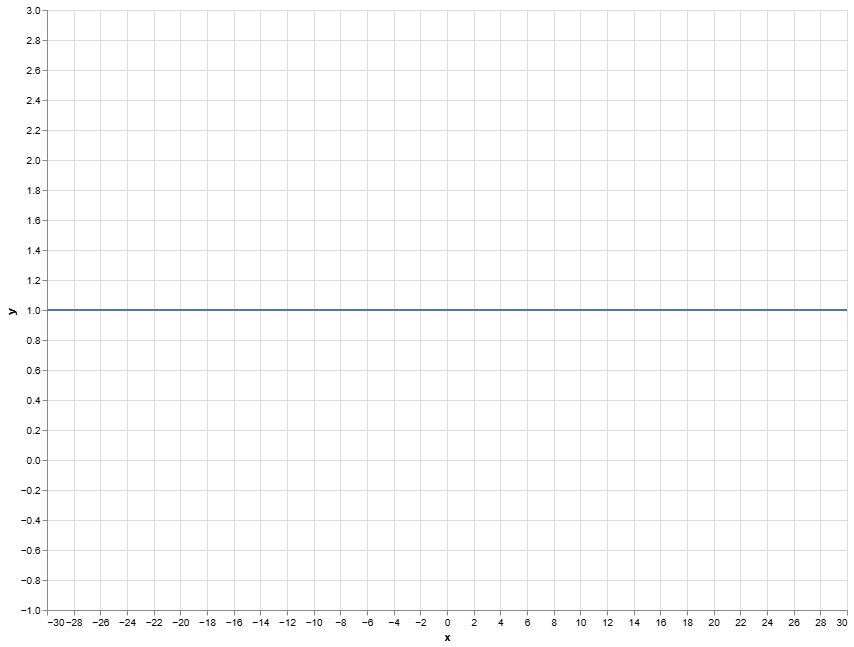
\includegraphics[width=\textwidth]{Imagens/x10_estavel.png}
        \caption{Comportamento estável no cálculo de \(x^{10} + 1 - x^{10}\) no intervalo \([-30, 30]\).}
        \label{fig:estavel}
    \end{minipage}
    \hfill
    \begin{minipage}{0.48\textwidth}
        \centering
        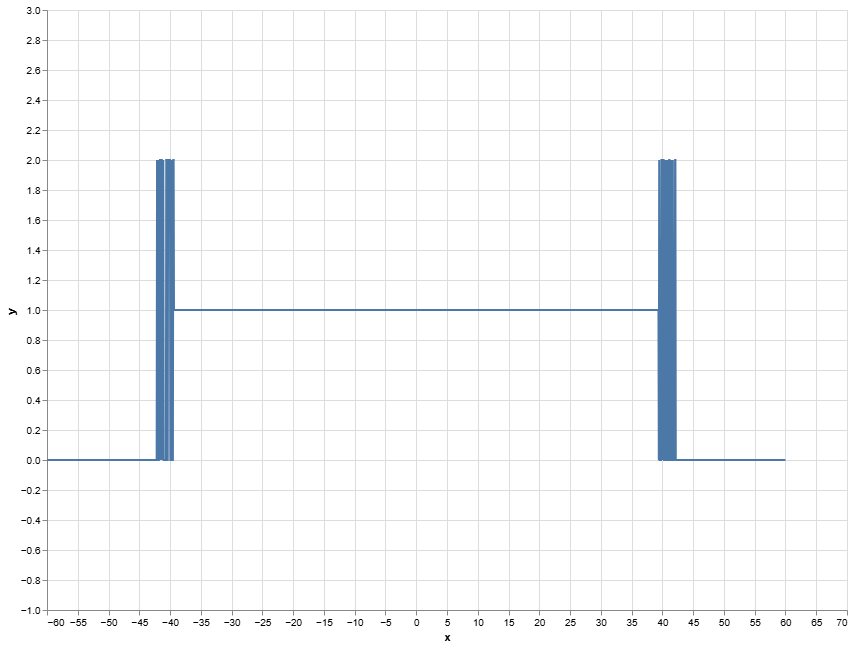
\includegraphics[width=\textwidth]{Imagens/x10_instavel.png}
        \caption{Comportamento instável no cálculo de \(x^{10} + 1 - x^{10}\) no intervalo \([-60, 60]\).}
        \label{fig:instavel}
    \end{minipage}
\end{figure}

\subsection{Perda de Significância em Somas}
Outro caso peculiar é a soma de um número muito grande com uma sequência de números pequenos. Dependendo da ordem em que as somas são realizadas, o número grande pode "mascarar" os pequenos, resultando em diferentes valores finais.

Por exemplo:
\[
S = 10^{8} + 10^{-1} + 10^{-2} + 10^{-3} + \ldots + 10^{-10}.
\]
Se somarmos primeiro o número grande (\(10^8\)) e depois os números pequenos, muitos destes podem ser ignorados devido à falta de precisão da mantissa. Por outro lado, ao somar os números pequenos antes, o valor final será mais próximo do esperado.

Para ilustrar, suponha a seguinte ordem de cálculo:
\begin{itemize}
    \item Caso 1: \(S = 10^{8} + (10^{-1} + 10^{-2} + \ldots + 10^{-10})\).
    \item Caso 2: \(S = (10^{-1} + 10^{-2} + \ldots + 10^{-10}) + 10^{8}\).
\end{itemize}
No primeiro caso, muitos números pequenos são ignorados devido ao arredondamento. No segundo, o somatório dos números pequenos é calculado antes de adicionar o número grande, preservando mais informações significativas.

\subsection{Discussão}
Esses exemplos destacam a importância da ordem das operações e da análise cuidadosa ao trabalhar com algoritmos numéricos. Técnicas como reordenação de cálculos e uso de formatos de precisão estendida podem ajudar a minimizar esses erros em contextos críticos.
